\section{Bilderkennung /-klassifikation} \label{chpt:Stand_der_Technik_Bilderkennung}
Ein bedeutender Bereich von maschinellem Lernen -- und damit Teilbereich von künstlicher Intelligenz -- ist die Bildklassifizierung (eng.: image classification). Diese Technik ermöglicht Computern die automatisierte Analyse und Kategorisierung beziehungsweise Zurodnung bestimmter Klassen von Bildern. Das Hauptziel eines Bildklassifizierungsalgorithmus liegt darin, einem Computer das Erkennen von Mustern und Merkmaln in Bildern beizubringen, um darauf basierend korrekt zu entscheiden, welcher vordefinierten Klasse das jeweilige Bild angehört.

Die Vielfalt von Bildklassifikations-Anwendungen ist enorm groß. Von medizinischen Möglichkeiten, wie Krebserkennung, bis hin zu Systemen für das Erkennen verschiedener Verkehrsteilnehmer, die sich in der Umgebung eines autonom fahrenden Kraftfahrzeuges bewegen. Durch das Einbringen von derartigen Lösungen können komplexe Aufgaben in nahezu Echtzeit gelöst und menschliche Fehler minimiert werden.

Der Bildklassifizierungsprozess besteht aus mehreren Schritten. Zunächst wird eine große Menge an Bildern gesammelt, welche in einen Trainings- und Testdatensatz aufgeteilt wird. Während Trainingsdaten für den Trainingsprozess verwendet werden, wird der Testdatensatz für die Validierung und Leistungsbewertung des trainierten Modells verwendet, um sicherzustellen, dass das Modell auch im Training ungesehene Daten richtig interpretiert. Während des Trainingsprozesses werden die Parameter des neuronalen Netzwerks meist mit einem überwachten Lernalgorithmus optimiert. Das Modell lernt die Identifizierung relevanter Merkmale um Bilder korrekt zu klassifizieren. Nach dem Training kann das Modell auf neue, nicht gesehene Bilder angewendet werden, um Vorhersagen über die Klassen-Zugehörigkeit des jeweiligen Inputs durchzuführen.

\subsection{Convolutional Neural Networks (CNN)}
Eine spezielle Art neuronaler Netzwerke sowie ein DeepLearning Algorithmus inspiriert von einem visuellen System lebender Organismen. (\cite[519]{balas_recent_2020}) Ein solches CNN ist variabel -- mit geringem Änderungsaufwand -- in jeglichen Bereichen der Bild- und Sprachverarbeitung einsetzbar. Das Training eines CNNs basiert meist auf überwachten Lernalgorithmen  (\ref{subsec:supervisedlearning}) und beansprucht durch die Diversität und Vielfalt der Daten enorm hohe Rechenleistung, geschuldet von meist großen Eingangsdaten und hoher Parameteranzahl des Modells.

Standardmäßig ist der Aufbau eines Convolutional Neural Networks für die Bildklassifizierung in zwei verschiedene Teile zu gliedern. Zum einen die Merkmalsextrahierung, welche wie folgt aufgebaut ist: einzelne oder mehrere Blöcke von Faltungs- und Vereinigungsschichten werden aneinander gereiht. Eine Faltungsschicht (eng.: convolutional layer) hat die Aufgabe, Merkmalsrepräsentationen zu erlernen, indem über einen Faltungskern mehrere Merkmalsbilder extrahiert werden. Um die Dimensionen zu reduzieren verwendet man die sogenannten Vereinigungsschichten (eng.: pooling layer), welche einen kleinen Bereich der Ausgabe einer Faltungsschicht entgegennehmen und diesen durch eine bestimmte Abtastung zu einer einzigen Ausgabe transformieren, wodurch auch nötige Parameter reduziert werden. Der zweite Teil des Netzwerks umfasst Schichten zur Klassifizierung des in Teil I generierten Outputs. Dazu gehören vollvermaschten Schichten, die zuvor extrahierte Rückgaben entgegennehmen, um darauf basierend ein Ergebnis -- und damit die endgültige Ausgabe des CNNs -- ableiten zu können.

Die Leistung eines solchen Netzwerks hängt von verschiedenen Faktoren ab, die für Optimierungszwecke verändert und verfeinert werden können. Dazu zählen beispielsweise Aktivierungsfunktionen, Normalisierungen, Verlustfunktionen, $\ldots$
\subsection{Merkmalextrahierung}
Die Mermalextrahierung (eng.: feature extraction) in einem neuronalen Netzwerk wird mit Hilfe von Faltungsschichten ermöglicht, welche den jeweiligen Input $I$ mit einem sogenannten Faltungskernel, der durch ein Raster diskreter Werte oder Zahlen beschrieben wird, filtern. Jeder Wert der Matrix legt eine bestimmte Gewichtung des Kernels fest, die während des Trainings angepasst werden kann. Initial gibt es die Möglichkeit das Training mit zufälligen Kernelgewichtungen zu starten oder selbst Werte zu definieren, abhängig von genutzter Methode.

Der vereinfachte \textit{Ablauf} einer Mermalextrahierung ist wie folgt: Der vordefinierte Filterkern der Größe $M \times N$ wird mit einer bestimmten Schrittgröße von Links nach Recht bewegt. Dabei wird während jedem Schritt ein gewichteter Durchschnitt berechnet, welcher den aktuellen Teil des Bildes repräsentiert. Dies wird bis Beendigung der gesamten Inputverarbeitung wiederholt. Die neuen Berechnungen speichert man in einer Matrix, die am Ende des Vorgangs das Resultat des Gesamtfilters darstellt. In der Regel wendet man eine nicht-lineare Aktivierungsfunktion auf die Ergebnisse der Faltung an, um Linerität in den Daten zu vermeiden.
\begin{figure}[H]
	\centering
	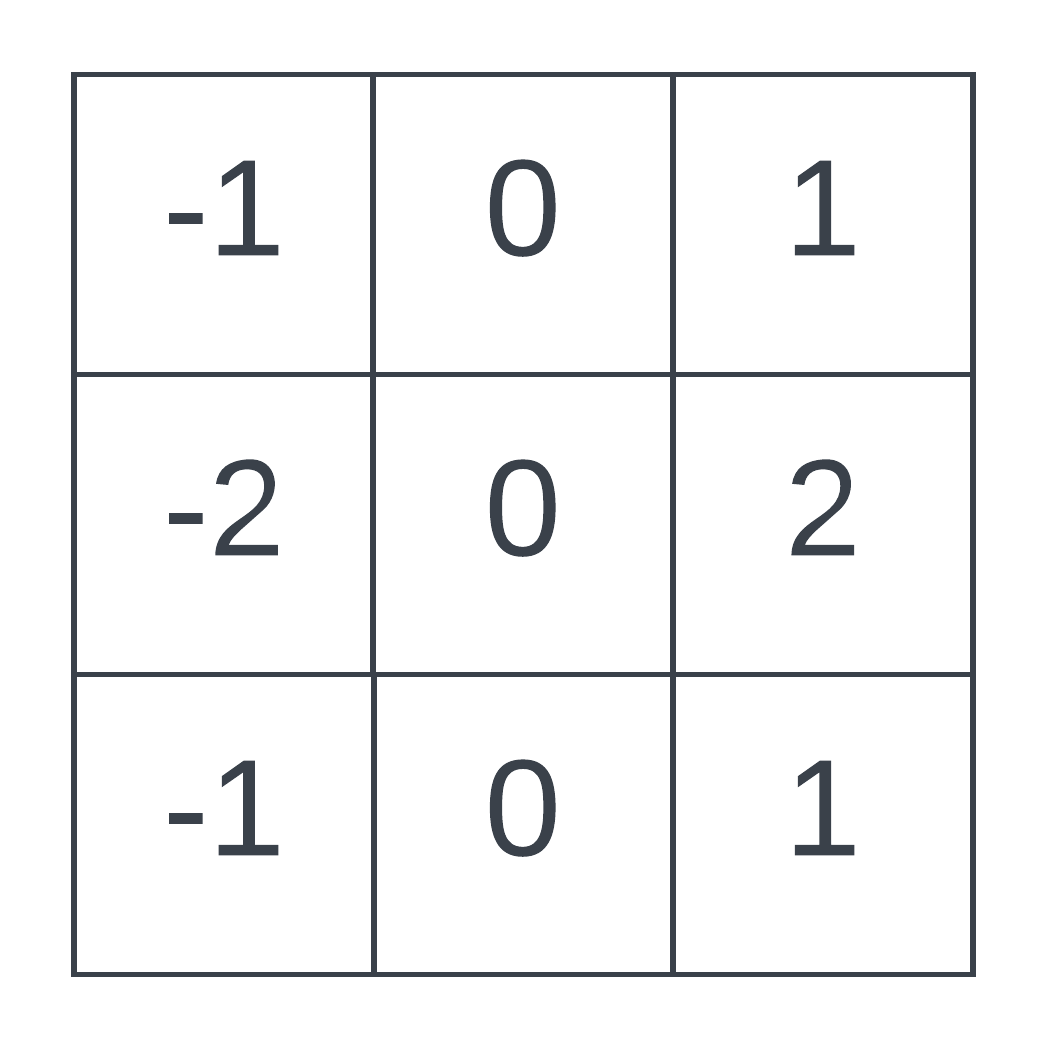
\includegraphics[width=0.2\linewidth]{Bilder/sobelfilter.png}
	\caption{Sobel-Filter (horizontal) mit vordefinierten Gewichtungen}
	\label{img:sobel}
\end{figure}
Ein Beispiel für einen gängigen Filterkern ist der horizontal angeordnete Sobel-Filter (Abbildung \ref{img:sobel}). Dieser wird verwendet, um horizontale Gradienten und Kanten in einem bestimmten Input zu detektieren. Der Filter berechnet bei jeder Position einen gewichteten Durchschnitt, womit im Laufe des Prozesses Kanten erkannt werden können. Dies ist der Fall, da die Gewichtungen des Filter so gewählt sind, dass diese besonders Empfindlich auf Veränderungen in horizontaler Richtung reagieren. Dadurch werden horizontale Kanten hervorgehoben, aber auch vertikale unterdrückt. Durch das Nutzen eines vertikalen Sobel-Filters ist das Verhalten umgekehrt. Nach Beenden des Durchgangs werden im Resultat, einer Feature-Map, die detektierten Kanten dargestellt.